\documentclass{article}
\usepackage[english]{babel}
\usepackage{geometry}
\geometry{tmargin=0.5in, margin=2.5cm}
\usepackage[utf8]{inputenc}
\usepackage{subcaption} 
\usepackage{tikz}
\usepackage{authblk}
\usepackage{float}
\usepackage{amsmath,bm}
\usepackage{amssymb}
\usepackage{amsthm}
\usepackage{mathtools}
\usepackage{cite}
\usepackage{verbatim}
\usepackage{indentfirst}
\usepackage{tikz-cd}
\usepackage{wrapfig}
\newtheorem{lemma}{Lemma}
\newtheorem{remark}{Remark}
\usepackage{mdframed}
\newmdtheoremenv{theorem}{Theorem}
\usepackage{mathrsfs}
\usepackage{url}
\usepackage{listings}

\title{Solving transient advection-diffusion-reaction equations by orthogonal-collocation method with special constraints via \texttt{Pyomo.dae}}

\author[1]{Guoxiang Grayson Tong}
\affil[1]{Ph.D. student, 
Department of Applied and Computational Mathematics and Statistics
}
\date{}

\begin{document}

\maketitle
\section{Abstract}
Numerically solving advection-diffusion-reaction systems has been an active research field for decades. In general, robust numerical approximations should be both well-behaved numerically, {\it{i.e.}} stability, fast convergence and {\it{etc}}, and also highly related to the real physics that the model represents. Unfortunately, most numerical techniques have their cons, either showing unsatisfactory numerical performance or violating certain physical/analytical laws. This project aims to further dive into this field of study by the combination of optimization tools and finite difference collocation methods. For certain scenarios, constraints like monotonicity, positivity of the solution will be added the simulation as to formulate a constrained optimization problem, which is usually not easily handled by the numerical scheme itself. In addition, the recent developed \texttt{pyomo.dae} will be utilized to realize the numerical examples. By the results, we found ......
\section{Introduction}
\indent \texttt{Python}-based \texttt{pyomo.dae}\cite{nicholson2018pyomo}, developed in recent years, provides convenient approaches to handle numerical optimization problems involving differential and algebraic equations. Explicitly, \texttt{pyomo.dae} prevails most existing optimization solvers by its support of PDE/ODE/DAE of arbitrary order, canonical or non-canonical forms, arbitrary domains and classical syntax of \texttt{Python}. Based on the knowledge learned in class and homework, this project will further investigate the power of \texttt{pyomo.dae} in solving PDE and PDE-constrained optimization problems.\par

\indent The PDEs of interest are the unsteady advection-diffusion-reaction equations:

\begin{alignat*}{2}
\displaystyle {\frac{\partial \phi}{\partial t}}  +  \mathbf{b} \cdot \nabla \phi - \nu \Delta \phi + c\phi &=f \quad \quad &&\text{in} \ \Omega \times [0,T]\\
\nabla \cdot \mathbf{b} &= 0 \quad \quad &&\text{in} \ \Omega \times [0,T] \\
\phi &= g \quad \quad &&\text{on} \ \Gamma_D \times [0,T] \\
\nabla \phi \cdot \mathbf{n} &= h \quad \quad &&\text{on} \ \Gamma_N \times [0,T]\\
\phi &= \phi_0 \quad \quad && \text{on} \ \Omega \times [0]
\end{alignat*}

We can also write the first PDE as a compact operator form: $\displaystyle {\frac{\partial \phi}{\partial t}}  + \mathcal{L}(\phi) =f$. This is also known as the scalar transport equations, where the scalar $\phi$ could be the concentration of a chemical, temperature, density, {\it{etc}}. The meanings of the above parameters are as: $\mathbf{b}$: the incompressible advection field, $\nu$: the diffusivity constant, $c$: the reaction constant, $f$: the source/sink. Besides, the problem is defined on the domain $\Omega \in \mathbb{R}^n$ with Dirichlet and Neumann boundaries $\Gamma_D$, $\Gamma_N \subset \partial \Omega \in \mathbb{R}^{n-1}$, respectively. In addition, to make this problem well-defined, we also need proper boundary conditions $g,h$ and initial condition $\phi_0$. This PDE is indeed a conservation law, which describes how a conserved quantity is transported in space time via macroscopic (momentum forces, advection) and microscopic (molecular diffusion, reaction) effect. \par

Numerically solving the above PDE can be achieved by many approaches: the finite element method\cite{evans2009enforcement}, the finite difference method\cite{stynes18}, the finite volume method\cite{lazarov1996finite}, the Lattice-Boltzmann method\cite{chai2013lattice} and the orthogonal collocation method\cite{biegler2010nonlinear} \cite{nicholson2018pyomo} that \texttt{pyomo.dae} unitizes to realize dynamic optimization. In general, robust numerical approximation of the above system should produce results satisfying both analytical and physical properties\cite{evans2009enforcement}. For example, the elliptic operator requires the global satisfaction of the maximum principle\cite{burman2005stabilized}\cite{evans2009enforcement}:
\begin{align*}
    \text{If} \ \mathcal{L}\phi \geq 0 \ &\text{in} \ \Omega, \ \text{then},\\
    \min_{\Bar{\Omega}} \phi &= \min_{\partial \Omega} \phi 
\end{align*}
For non-negative forcing, the above directly leads to the non-negative constraint:
\begin{equation*}
    \min_{\Bar{\Omega}} \phi = 0
\end{equation*}
This condition is also closely related to the real physics, {\it{i.e.}}, we are not expecting negative density and concentration. Furthermore, we still need the numerical solution to be monotone, in the cases of no reaction and forcing, since in certain applications, oscillatory results clearly violates the second law of the thermodynamics. However, most numerical methods are not oscillation-free because of various reasons\cite{john2018finite}. Oscillations usually bring nonphysical over/undershoots, especially in the presence of of internal and boundary layers.  In this project, we intend to resolve the aformentioned issues by optimization techniques. We classify the satisfactions of ``discrete maximum principle, non-negativity and monotonicity" as \textbf{special constraints}.

\section{Model development}
Enforcing special constraints to the steady advection-diffusion system has been well-studied in the past by finite-element based variational multiscale method\cite{evans2009enforcement}. This project aims to extend this idea to finite-difference based orthogonal collocation methods via \texttt{pyomo.dae} (upon finishing, the code of this project will be opened to public as the footnote below\footnote{\url{https://github.com/Grayson3455/ADR-pyomo.dae}}). Further, transient problem and additional reaction term will be considered. Namely, we are interested in the following discrete optimization problem:
\begin{alignat*}{1}
\text{Find $\phi_h$ in $\Bar{\Omega}_h\times[0 ,T]$, s.t.} \\
    \displaystyle {\frac{\partial \phi_h}{\partial t}}  + \mathcal{L}(\phi_h) &= f \\
    \phi_h|_{\Gamma_D} &= g_h\\
    \phi_h|_{t=0} &= \phi_{0,h}\\
    \min_{\Bar{\Omega}_h} \phi_h &= 0 \\
    \min_{\Bar{\Omega}_h} \phi_h &= \min_{\partial \Omega_h} \phi_h \\
    sgn(\nabla \phi_h) \geq 0 \ &\text{or} \ sgn(\nabla \phi_h) \leq 0
\end{alignat*}
Compared to the general model above, we will consider pure Dirichlet boundary value problem for simplicity. Besides, we will only consider the 2D problem. 
Note that this optimization will have both equality and inequality constraints, partial differential equation and algebraic equation constraints. The PDE itself is linear and we will consider only the constant advective velocity $\mathbf{b}$, diffusivity $\nu$ and reaction parameter $c$. In addition, the positivity, discrete maximum principle and monotonicity are to be implemented as last three constraints above, respectively.
\section{Mathematical analysis}
Write out the finite difference collocation schemes for the ADR system and apply constrained optimization theory to it.
\section{Numerical examples}
\subsection{Smooth problem}
We first test the functionality of \texttt{pyomo.dae} by solving advection-diffusion-reaction equations with known solutions. This is often referred as the test by manufactured solutions, {\it{i.e.}}, we design a solution profile $\phi(x,y)$ and then plug it to the PDE to solve for the source/sink term $f$. The example we followed was originally proposed by \cite{burman2004edge}, which is characterized by a hyperbolic tangent distribution only in $x-$direction: $$\phi(x,y) = \frac{1}{2} (1-\text{tanh}(\frac{x - 0.5}{\lambda}))$$
With the parameters $\mathbf{b} = (1,0)$, $\nu=10^{-5}, c = 1$, $\lambda = 0.05$. Note that the magnitude of $\lambda$ controls the slope of the hyperbolic function, which brings an interior layer near $x=0.5$. 
\subsubsection{Case1: Steady advection-diffusion-reaction equation}
Solved by the finite difference collocation solver provided in $\texttt{pyomo.dae}$, we have the following results:
\begin{figure}[H]
\centering
   	 \begin{subfigure}[b]{0.49\textwidth}
   	 	\centering
		\includegraphics[height=3in]{fig/steady-adr-smooth.png}
		\caption{\centering{Solution profile}}
		\label{s-adr}
	\end{subfigure}
	\begin{subfigure}[b]{0.49\textwidth}
   	 	\centering
		\includegraphics[height=3in]{fig/steady-adr-smooth-error.png}
		\caption{\centering{Nodal error distribution}}
		\label{se-adr}
	\end{subfigure}

	\caption{\texttt{pyomo} solution of the manufactured advection-diffusion-reaction problem}
	\label{f1}
\end{figure}

Note that with only 9 finite elements and 3 collocation points each, we still have a decent approximation. Also, it's clear the error peaks near the interior layer, where sharp solution gradient brings less accuracy by polynomial-based numerical approximations.

\subsubsection{Case2: Unsteady advection-diffusion-reaction equation}
Without creating the time-dependent part, we initiated a parabolic function as the initial condition and start time-marching. Theoretically, the steady state will be reached by a few time steps.
\subsection{Non-smooth problem}
So far, we did not see any spurious oscillations, over/undershoots triggered by numerical instabilities. Besides the robust numerical property provided by the collocation scheme, the smoothness assumption of the problem also makes a contribution. In this section, we will consider the so-called skewed advection problem, where the special structure of the boundary conditions brings discontinuity and immediately creates a singularity-perturbed problem.
\subsubsection{Case1: Steady advection-diffusion-reaction equation}
\begin{figure}[H]
   	 	 \begin{center}
			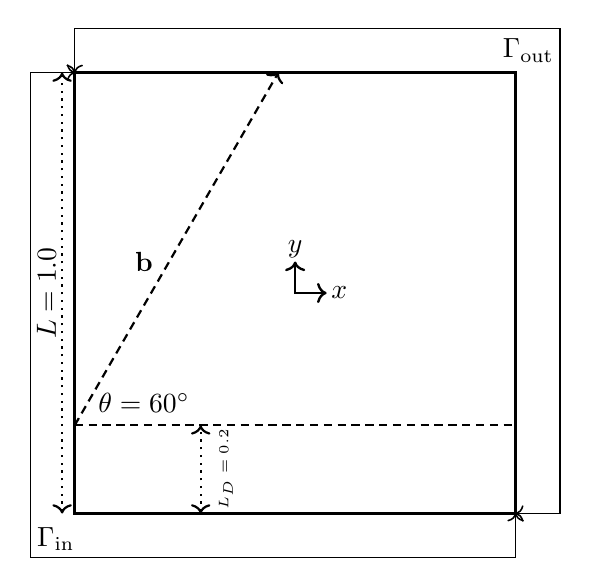
\begin{tikzpicture}[scale = 0.8]
			% coordinate_sys
			\draw [<->][line width=0.3mm, black]  (3.5,4) -- (3.5,3.5) -- (4,3.5) ;
			\node at (3.5,4.2) {$y$};
			\node at(4.2,3.5) {$x$};
	
			%box 
			\draw[black, very thick] (0,0) rectangle (7,7);
			\draw [line width=0.5mm, black, thick, densely dashed] (0,1.4) -- (7,1.4) ;
			\draw [<->][line width=0.5mm, black, thick, dotted ] (2,0) -- (2,1.4) ;
			\node [rotate=90] at (2.4,0.7) {\tiny{$L_D = 0.2$}};
			\draw [<->][line width=0.5mm, black, thick, dotted ] (-0.2,0) -- (-0.2,7) ;
			\node [rotate=90] at (-.45,3.5) {$L = 1.0$};
			% advec
			\draw [black, thick] (0,1.4) -- (0,0) -- (7,0) ;
			\draw [->][black, thick, densely dashed] (0,1.4) -- ++(60:6.48cm);
			\node at(1.1,1.75) {$\theta = 60^\circ$};
			\node at(1.1,4) {$\mathbf{b}$};
			% in and out
			\draw [<->][line width=0.2mm, black] (0, 7)-- (-.7,7) -- (-0.7,-.7) -- (7,-0.7) -- (7,0); %in
			\node [align=left] [text=black] at (-.3,-.4) {$\Gamma_{\text{in}}$};
			\draw [<->][line width=0.2mm, black] (0,7) -- (0, 7.7) -- (7.7,7.7) -- (7.7,0)  -- (7,0);  %out
			\node [align=left] [text=black] at (7.2,7.35) {$\Gamma_{\text{out}}$};
			\end{tikzpicture}
			\caption{Sketch of the skewed advection model}
			\end{center}
\end{figure}
\subsubsection{Case2: Unsteady advection-diffusion-reaction equation}
\section{Conclusions}
\bibliographystyle{plain}
\bibliography{ref}{}

\section*{Appendix 1: Computer code(steady ADR example)}
\begin{lstlisting}
from pyomo.environ import *
from pyomo.dae import *
import numpy as np
from matplotlib import pyplot as plt

# space-time variables
m      = ConcreteModel()
m.x    = ContinuousSet(bounds = (0,1))
m.y    = ContinuousSet(bounds = (0,1))
m.phi  = Var(m.x, m.y)

# define derivative variables
m.DphiDx   = DerivativeVar(m.phi, wrt = m.x)
m.DphiDy   = DerivativeVar(m.phi, wrt = m.y)
m.DphiDx_2 = DerivativeVar(m.phi, wrt = (m.x, m.x))
m.DphiDy_2 = DerivativeVar(m.phi, wrt = (m.y, m.y))

# define PDE parameters
m.c 	= Param(initialize = 1.0)  # the reaction constant
m.nu    = Param(initialize = 1e-5) # the diffusivity
m.bx    = Param(initialize = 1.0)  # the advection velocity, x-component
m.by    = Param(initialize = 0.0)  # the advection velocity, y-component
m.lmd     = Param(initialize = 0.05) # slope of manufactured solution 

# create lambda function for manufactured solutions
u_e    	= lambda x : 0.5* ( 1.0 - np.tanh((x - 0.5)/value(m.lmd)) ) 
du_e    = lambda x : -1.0/(2.0*value(m.lmd)) \
		 * (1.0/np.cosh((x-0.5)/value(m.lmd)))**2
du_e2   = lambda x : 1.0/value(m.lmd)/value(m.lmd) * \
		 (1.0/np.cosh((x-0.5)/value(m.lmd)))**2 * np.tanh((x - 0.5)/value(m.lmd))
f       = lambda x,y : du_e(x) - value(m.nu) * du_e2(x) + value(m.c)*u_e(x) 

# define adr pde, i: x, j: y
def ADR_pde(m,i,j):
	if i == 0 or i  == 1: # boundary conditions to be implemented, no constraints
		return Constraint.Skip
	return m.bx * m.DphiDx[i,j] + m.by * m.DphiDy[i,j]- m.nu*m.DphiDx_2[i,j] \
	- m.nu*m.DphiDy_2[i,j]  + m.c*m.phi[i,j] == f(i,j)
m.pde = Constraint(m.x, m.y, rule = ADR_pde )  

# left boundary condition [phi = 1 @ x = 0]
def BC1(m,j):
	return m.phi[0,j] == 1.0
m.BCx_0 = Constraint(m.y, rule = BC1)

# right boundary condition [phi = 0 @ x = 1]
def BC2(m,j):
	return m.phi[1,j] == 0.0 
m.BCx_1 = Constraint(m.y, rule = BC2)

# trivial obj
m.obj = Objective(expr = 1)

# discretization and solve
discretizer = TransformationFactory('dae.collocation')
discretizer.apply_to(m,nfe=9,ncp=4,wrt=m.x)
discretizer.apply_to(m,nfe=9,ncp=4,wrt=m.y)

solver = SolverFactory('ipopt')
results = solver.solve(m, tee=True) 

\end{lstlisting}
\end{document}
